\documentclass[14pt]{extbook}
\usepackage{multicol, enumerate, enumitem, hyperref, color, soul, setspace, parskip, fancyhdr} %General Packages
\usepackage{amssymb, amsthm, amsmath, latexsym, units, mathtools} %Math Packages
\everymath{\displaystyle} %All math in Display Style
% Packages with additional options
\usepackage[headsep=0.5cm,headheight=12pt, left=1 in,right= 1 in,top= 1 in,bottom= 1 in]{geometry}
\usepackage[usenames,dvipsnames]{xcolor}
\usepackage{dashrule}  % Package to use the command below to create lines between items
\newcommand{\litem}[1]{\item#1\hspace*{-1cm}\rule{\textwidth}{0.4pt}}
\pagestyle{fancy}
\lhead{Progress Quiz 4}
\chead{}
\rhead{Version C}
\lfoot{5346-5907}
\cfoot{}
\rfoot{Summer C 2021}
\begin{document}

\begin{enumerate}
\litem{
Solve the linear equation below. Then, choose the interval that contains the solution.\[ \frac{-7x + 6}{8} - \frac{5x -8}{2} = \frac{-5x -4}{7} \]\begin{enumerate}[label=\Alph*.]
\item \( x \in [0.1, 1.2] \)
\item \( x \in [1.7, 3.1] \)
\item \( x \in [-2.6, -0.4] \)
\item \( x \in [6.2, 8] \)
\item \( \text{There are no real solutions.} \)

\end{enumerate} }
\litem{
Solve the equation below. Then, choose the interval that contains the solution.\[ -19(14x + 6) = -3(4x -16) \]\begin{enumerate}[label=\Alph*.]
\item \( x \in [-0.77, -0.57] \)
\item \( x \in [-0.34, -0.25] \)
\item \( x \in [-0.25, -0.17] \)
\item \( x \in [0.18, 0.4] \)
\item \( \text{There are no real solutions.} \)

\end{enumerate} }
\litem{
First, find the equation of the line containing the two points below. Then, write the equation in the form $ y=mx+b $ and choose the intervals that contain $m$ and $b$.\[ (2, 8) \text{ and } (4, -2) \]\begin{enumerate}[label=\Alph*.]
\item \( m \in [-12, -4] \hspace*{3mm} b \in [4, 10] \)
\item \( m \in [-12, -4] \hspace*{3mm} b \in [-6, -2] \)
\item \( m \in [-12, -4] \hspace*{3mm} b \in [-20, -14] \)
\item \( m \in [4, 6] \hspace*{3mm} b \in [-26, -20] \)
\item \( m \in [-12, -4] \hspace*{3mm} b \in [17, 19] \)

\end{enumerate} }
\litem{
Write the equation of the line in the graph below in Standard Form $Ax+By=C$. Then, choose the intervals that contain $A, B, \text{ and } C$.
\begin{center}
    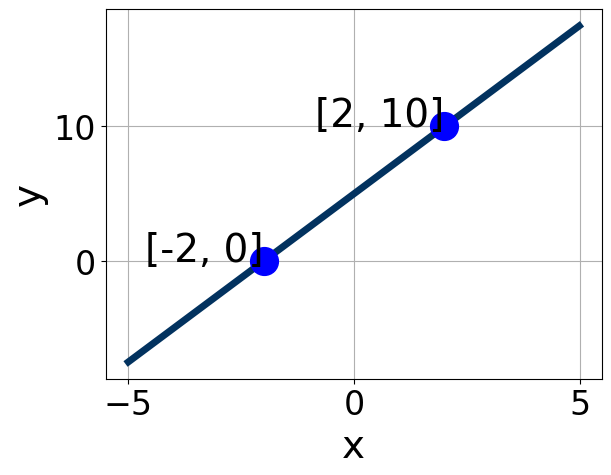
\includegraphics[width=0.5\textwidth]{../Figures/linearGraphToStandardCopyC.png}
\end{center}
\begin{enumerate}[label=\Alph*.]
\item \( A \in [-2.5, -1.5], \hspace{3mm} B \in [0.1, 1.11], \text{ and } \hspace{3mm} C \in [4, 7] \)
\item \( A \in [-6, -3], \hspace{3mm} B \in [1.49, 3.66], \text{ and } \hspace{3mm} C \in [9, 11] \)
\item \( A \in [-2.5, -1.5], \hspace{3mm} B \in [-1.41, -0.53], \text{ and } \hspace{3mm} C \in [-7, -4] \)
\item \( A \in [4, 8], \hspace{3mm} B \in [1.49, 3.66], \text{ and } \hspace{3mm} C \in [9, 11] \)
\item \( A \in [4, 8], \hspace{3mm} B \in [-3.93, -1.4], \text{ and } \hspace{3mm} C \in [-12, -7] \)

\end{enumerate} }
\litem{
Find the equation of the line described below. Write the linear equation in the form $ y=mx+b $ and choose the intervals that contain $m$ and $b$.\[ \text{Parallel to } 7 x - 8 y = 9 \text{ and passing through the point } (7, 8). \]\begin{enumerate}[label=\Alph*.]
\item \( m \in [0.77, 0.95] \hspace*{3mm} b \in [0.05, 1.77] \)
\item \( m \in [0.77, 0.95] \hspace*{3mm} b \in [-2.58, -0.48] \)
\item \( m \in [0.98, 1.67] \hspace*{3mm} b \in [1.55, 2.01] \)
\item \( m \in [-1.19, -0.36] \hspace*{3mm} b \in [13.58, 15.14] \)
\item \( m \in [0.77, 0.95] \hspace*{3mm} b \in [1.55, 2.01] \)

\end{enumerate} }
\litem{
Solve the equation below. Then, choose the interval that contains the solution.\[ -13(17x -2) = -12(-9x -4) \]\begin{enumerate}[label=\Alph*.]
\item \( x \in [0.65, 0.74] \)
\item \( x \in [-0.28, -0.21] \)
\item \( x \in [-0.18, 0.14] \)
\item \( x \in [0.03, 0.28] \)
\item \( \text{There are no real solutions.} \)

\end{enumerate} }
\litem{
Find the equation of the line described below. Write the linear equation in the form $ y=mx+b $ and choose the intervals that contain $m$ and $b$.\[ \text{Parallel to } 5 x - 4 y = 4 \text{ and passing through the point } (-8, 5). \]\begin{enumerate}[label=\Alph*.]
\item \( m \in [1.14, 1.98] \hspace*{3mm} b \in [14, 18] \)
\item \( m \in [-2, -0.92] \hspace*{3mm} b \in [-9, -1] \)
\item \( m \in [1.14, 1.98] \hspace*{3mm} b \in [-16, -12] \)
\item \( m \in [0.37, 0.85] \hspace*{3mm} b \in [14, 18] \)
\item \( m \in [1.14, 1.98] \hspace*{3mm} b \in [10, 14] \)

\end{enumerate} }
\litem{
Write the equation of the line in the graph below in Standard Form $Ax+By=C$. Then, choose the intervals that contain $A, B, \text{ and } C$.
\begin{center}
    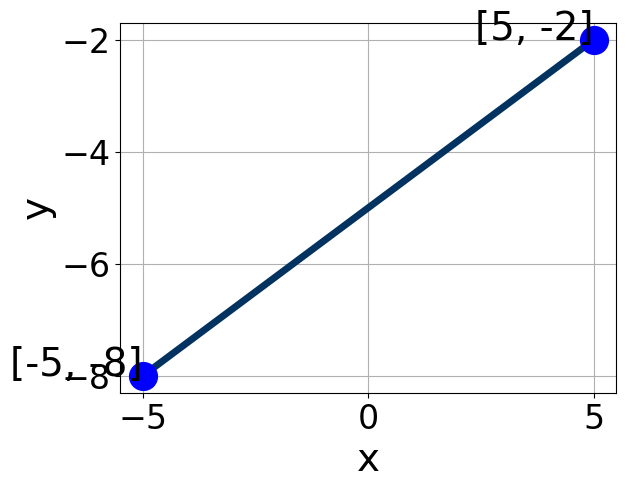
\includegraphics[width=0.5\textwidth]{../Figures/linearGraphToStandardC.png}
\end{center}
\begin{enumerate}[label=\Alph*.]
\item \( A \in [-7.6, -1.2], \hspace{3mm} B \in [1.2, 5.1], \text{ and } \hspace{3mm} C \in [-29, -23] \)
\item \( A \in [-1.1, 1.2], \hspace{3mm} B \in [-2, -0.4], \text{ and } \hspace{3mm} C \in [4, 6] \)
\item \( A \in [2.1, 5.6], \hspace{3mm} B \in [-5.8, -2.8], \text{ and } \hspace{3mm} C \in [19, 34] \)
\item \( A \in [2.1, 5.6], \hspace{3mm} B \in [1.2, 5.1], \text{ and } \hspace{3mm} C \in [-29, -23] \)
\item \( A \in [-1.1, 1.2], \hspace{3mm} B \in [-0.7, 1.5], \text{ and } \hspace{3mm} C \in [-10, 2] \)

\end{enumerate} }
\litem{
Solve the linear equation below. Then, choose the interval that contains the solution.\[ \frac{-8x + 8}{3} - \frac{-8x -8}{5} = \frac{-8x + 7}{4} \]\begin{enumerate}[label=\Alph*.]
\item \( x \in [-0.6, 0.1] \)
\item \( x \in [-10.2, -7.4] \)
\item \( x \in [-3.2, -2.2] \)
\item \( x \in [0.5, 1.1] \)
\item \( \text{There are no real solutions.} \)

\end{enumerate} }
\litem{
First, find the equation of the line containing the two points below. Then, write the equation in the form $ y=mx+b $ and choose the intervals that contain $m$ and $b$.\[ (-3, 10) \text{ and } (-7, -9) \]\begin{enumerate}[label=\Alph*.]
\item \( m \in [-0.25, 6.75] \hspace*{3mm} b \in [10, 21] \)
\item \( m \in [-0.25, 6.75] \hspace*{3mm} b \in [-31.25, -22.25] \)
\item \( m \in [-0.25, 6.75] \hspace*{3mm} b \in [-7, 2] \)
\item \( m \in [-0.25, 6.75] \hspace*{3mm} b \in [23.25, 25.25] \)
\item \( m \in [-4.75, 1.25] \hspace*{3mm} b \in [-42.25, -40.25] \)

\end{enumerate} }
\end{enumerate}

\end{document}